\section{Bewijzen}

\begin{answer} % 3.1
Bewijs met de boommethode dat:
\begin{enumerate}[label=\textit{\alph*.}]
%a:
\item $p\vdash p$\\
antwoord: Laat zien dat de negatie van de conclusie tot onvervulbaarheid leidt om het logisch gevolg aan te tonen:
\begin{center}
    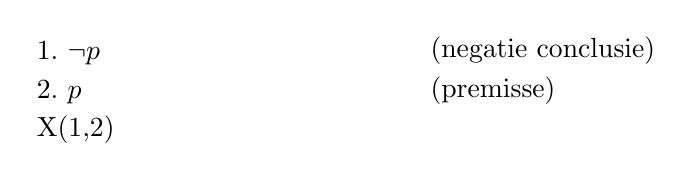
\begin{tikzpicture}[anchor=south west]
    \node at (2, 3) {$1.\ \neg p$};\node at (7,3) {(negatie conclusie)};
    \node at (2, 2.5) {$2.\ p$};\node at (7, 2.5) {(premisse)};
    \node at (2, 2) {X(1,2)};
    \end{tikzpicture}
\end{center}
De boom sluit, dus de combinatie van premisse met de negatie van de conclusie is onvervulbaar. Het logisch gevolg is dus geldig.
%b:
\item $p\wedge q\vdash q$\\
antwoord: Laat wederom zien dat de negatie van de conclusie tot onvervulbaarheid leidt:
\begin{center}
    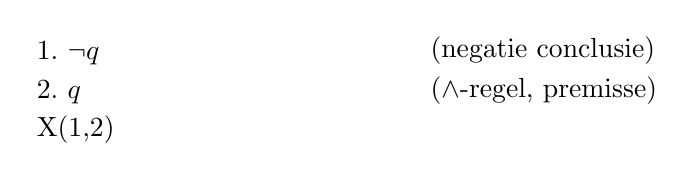
\begin{tikzpicture}[anchor=south west]
    \node at (2, 3) {$1.\ \neg q$}; \node at (7,3) {(negatie conclusie)};
    \node at (2, 2.5) {$2.\ q$}; \node at (7, 2.5) {($\wedge$-regel, premisse)};
    \node at (2, 2) {X(1,2)};
    \end{tikzpicture}
\end{center}
De boom sluit, dus de combinatie van premisse met de negatie van de conclusie is onvervulbaar. Het logisch gevolg is dus geldig.
%c:
\item $p\rightarrow q\vdash \neg p\vee q$\\
antwoord: Idem, check premissen met negatie van conclusie op vervulbaarheid:
\begin{center}
    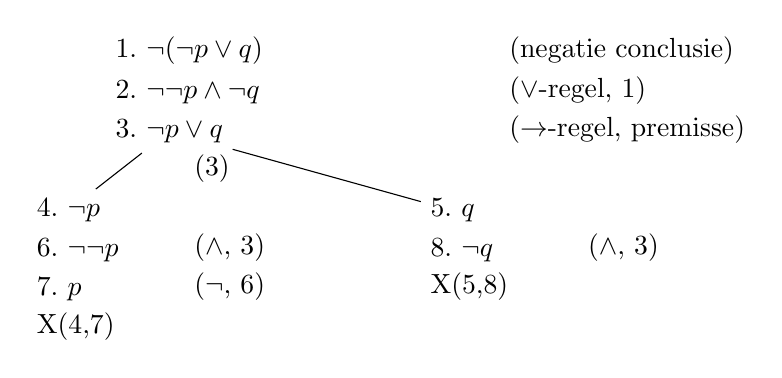
\begin{tikzpicture}[anchor=south west]
    \node at (2,5) {$1.\ \neg(\neg p\vee q)$};\node at (7,5) {(negatie conclusie)};
    \node at (2, 4.5) {$2.\ \neg\neg p\wedge\neg q$};\node at (7, 4.5) {($\vee$-regel, 1)};
    \node at (2, 4) (p1) {$3.\ \neg p\vee q$}; \node at (7, 4) {($\rightarrow$-regel, premisse)};
    \node at (1, 3) (p2) {$4.\ \neg p$}; \node at (6, 3) (p3) {$5.\ q$};
    \draw (p2) -- (p1) -- (p3);
    \node at (3, 3.5) {$(3)$};
    %% branch 1
    \node at (1, 2.5) {$6.\ \neg\neg p$};\node at (3, 2.5) {($\wedge$, 3)};
    \node at (1, 2) {$7.\ p$}; \node at (3, 2) {($\neg$, 6)};
    \node at (1, 1.5) {X(4,7)};
    %% branch 2
    \node at (6, 2.5) {$8.\ \neg q$}; \node at (8,2.5) {($\wedge$, 3)};
    \node at (6, 2) {X(5,8)};
    \end{tikzpicture}
\end{center}
Alle takken sluiten, dus het logisch gevolg is geldig.
%d:
\item $\neg p\vdash p\rightarrow q$\\
antwoord: Idem, check premissen met negatie van conclusie op vervulbaarheid:
\begin{center}
    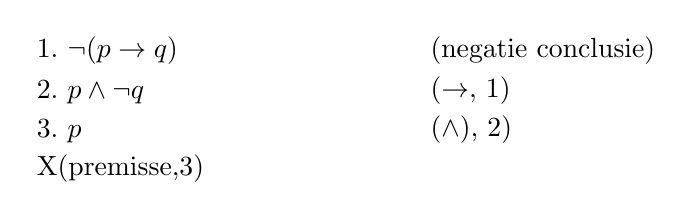
\begin{tikzpicture}[anchor=south west]
    \node at (2, 5) {$1.\ \neg(p\rightarrow q)$};\node at (7,5) {(negatie conclusie)};
    \node at (2, 4.5) {$2.\ p\wedge\neg q$}; \node at (7,4.5) {($\rightarrow$, 1)};
    \node at (2, 4) {$3.\ p$}; \node at (7, 4) {($\wedge$), 2)};
    \node at (2, 3.5) {X(premisse,3)};
    \end{tikzpicture}
\end{center}
Alle takken sluiten, dus ook dit logisch gevolg is geldig.
%e:
\item $\neg(p\vee q)\vdash p\rightarrow q$\\
antwoord: Idem, check premissen met negatie van conclusie op vervulbaarheid:
\begin{center}
    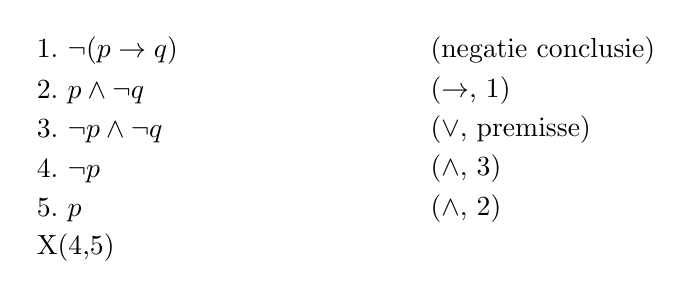
\begin{tikzpicture}[anchor=south west]
    \node at (2,5) {$1.\ \neg(p\rightarrow q)$};\node at (7,5) {(negatie conclusie)};
    \node at (2,4.5) {$2.\ p\wedge\neg q$}; \node at (7,4.5) {($\rightarrow$, 1)};
    \node at (2, 4) {$3.\ \neg p\wedge\neg q$};\node at (7,4) {($\vee$, premisse)};
    \node at (2, 3.5) {$4.\ \neg p$}; \node at (7,3.5) {($\wedge$, 3)};
    \node at (2, 3) {$5.\ p$};\node at (7,3) {($\wedge$, 2)};
    \node at (2,2.5) {X(4,5)};
    \end{tikzpicture}
\end{center}
Alle takken sluiten, dus logisch gevolg is geldig.
\end{enumerate}
\end{answer}


\begin{answer} % 3.2
Ga voor elk van de onderstaande beweringen na of dat deze juist danwel onjuist is. Geef in het eerste geval een bewijs met behulp van de boommethode. Construeer in het tweede geval een \textit{tegenvoorbeeld}.
\begin{enumerate}[label=\textit{\alph*.}]
% a:
\item $p\rightarrow q$ is een tautologie (d.w.z. $\vdash p\rightarrow q$). \\ 
antwoord:
\begin{center}
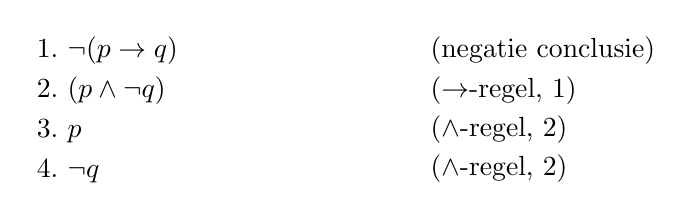
\begin{tikzpicture}[anchor=south west]
\node at (2,6) {$1.\ \neg (p\rightarrow q)$}; \node at (7,6) {(negatie conclusie)};
\node at (2,5.5) {$2.\ (p \land \neg q$)}; \node at (7,5.5) {($\rightarrow$-regel, 1)};
\node at (2,5) {$3.\  p$}; \node at (7,5) {($\land$-regel, 2)};
\node at (2,4.5) {$4.\ \neg q$}; \node at (7,4.5) {($\land$-regel, 2)};
\end{tikzpicture}
\end{center}
Er is een tak die niet sluit, dus er is een tegenvoorbeeld mogelijk. Het tegenvoorbeeld volgt uit 3 en 4: $p=1$ en $q=0$.
%b:
\item $p\rightarrow p$ is een tautologie (d.w.z. $\vdash p\rightarrow p$).\\
antwoord:
\begin{center}
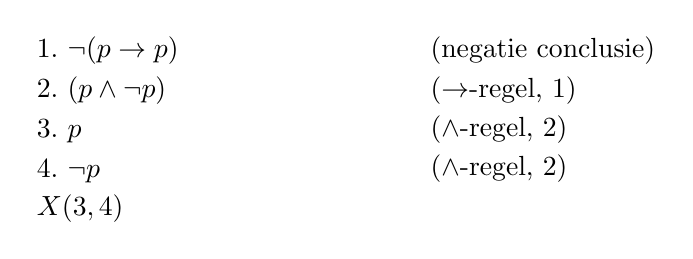
\begin{tikzpicture}[anchor=south west]
\node at (2,6) {$1.\ \neg (p\rightarrow p)$}; \node at (7,6) {(negatie conclusie)};
\node at (2,5.5) {$2.\ (p \land \neg p$)}; \node at (7,5.5) {($\rightarrow$-regel, 1)};
\node at (2,5) {$3.\  p$}; \node at (7,5) {($\land$-regel, 2)};
\node at (2,4.5) {$4.\ \neg  p$}; \node at (7,4.5) {($\land$-regel, 2)};
\node at (2,4) {$X(3,4)$};
\end{tikzpicture}
\end{center}
De boom sluit, dus $\neg (p\rightarrow p)$ is onvervulbaar. Daarmee is bewezen dat $\vdash p\rightarrow p$.
%c:
\item $p\leftrightarrow p$ is een tautologie (d.w.z. $\vdash p\leftrightarrow p$). \\ 
antwoord:
\begin{center}
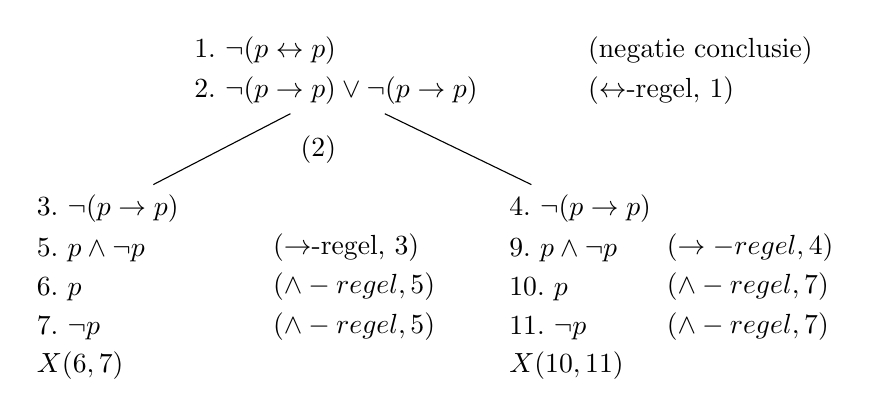
\begin{tikzpicture}[anchor=south west]
\node at (2,6) {$1.\ \neg(p\leftrightarrow p)$}; \node at (7,6) {(negatie conclusie)};
\node at (2,5.5) (p1) {$2.\ \neg(p\rightarrow p)\lor\neg(p\rightarrow p)$}; \node at (7,5.5) {($\leftrightarrow$-regel, 1)};
\node at (0,4) (p2) {$3.\  \neg (p \rightarrow p)$}; \node at (6,4) (p3) {$4.\ \neg(p \rightarrow p)$};
\draw (p2) -- (p1) -- (p3);
\node at (3.35, 4.75) {$(2)$};
%branch 1
\node at (0,3.5) {$5.\ p\land \neg p$}; \node at (3,3.5) {($\rightarrow$-regel, 3)};
\node at (0,3) {$6.\ p$}; \node at (3,3) {($\land-regel, 5)$};
\node at (0,2.5) {$7.\ \neg p$}; \node at (3,2.5) {($\land-regel, 5)$};
\node at (0,2) {$X(6,7)$}; 
%branch 2
\node at (6,3.5) {$9.\ p\land \neg p$}; \node at (8,3.5) {($\rightarrow-regel, 4)$};
\node at (6,3) {$10.\ p$}; \node at (8,3) {($\land-regel, 7)$};
\node at (6,2.5) {$11.\ \neg p$}; \node at (8,2.5) {($\land-regel, 7)$};
\node at (6,2) {$X(10,11)$}; 
\end{tikzpicture}
\end{center}
Alle takken sluiten, dus $\neg(p\leftrightarrow p)$ is onvervulbaar. Daarmee is bewezen dat $\vdash p \leftrightarrow p$.
%d:
\item $p\wedge\neg q$ is een contradictie (d.w.z $\not\vdash p\wedge\neg q$ ofwel $\vdash\neg(p\wedge\neg q)$). \\ 
antwoord:\\
Laat zien dat $p\wedge\neg q$ onvervulbaar is:
\begin{center}
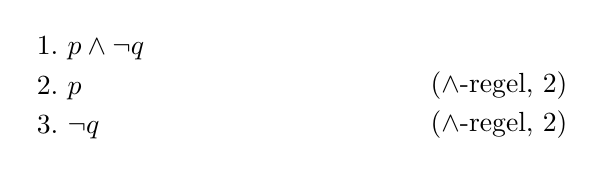
\begin{tikzpicture}[anchor=south west]
\node at (2,5.5) {$1.\ p\land \neg q$}; %\node at (7,5.5) {($\neg$-regel, 1)};
\node at (2,5) {$2.\ p$}; \node at (7,5) {($\land$-regel, 2)};
\node at (2,4.5) {$3.\ \neg q$}; \node at (7,4.5) {($\land$-regel, 2)};
\end{tikzpicture}
\end{center}
Er is een tak die niet sluit, $p\wedge\neg q$ is dus vervulbaar en daardoor geen contradictie ($p\wedge\neg q$ is immers waar als $p=1$ en $q=0$).
%e:
\item $p\wedge\neg p$ is een contradictie (d.w.z. $\not\vdash p\wedge\neg p$). \\
antwoord:\\
$\not\vdash p\wedge\neg p$ bewijzen is hetzelfde als bewijzen dat $p\wedge\neg p$ onvervulbaar is:
\begin{center}
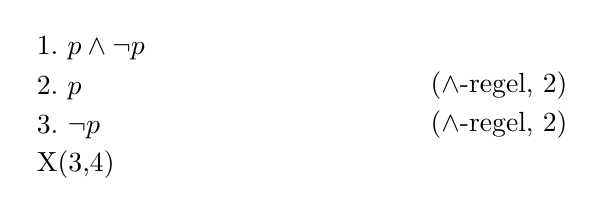
\begin{tikzpicture}[anchor=south west]
\node at (2,5.5) {$1.\ p\land \neg p$}; %\node at (7,5.5) {($\neg$-regel, 1)};
\node at (2,5) {$2.\ p$}; \node at (7,5) {($\land$-regel, 2)};
\node at (2,4.5) {$3.\ \neg p$}; \node at (7,4.5) {($\land$-regel, 2)};
\node at (2,4) {X(3,4)};
\end{tikzpicture}
\end{center}
Alle takken sluiten, dus $p\wedge\neg p$ is onvervulbaar; dat wil zeggen, $p\wedge\neg p$ is een contradictie.
%f:
\item $p\leftrightarrow\neg p$ is een contradictie (d.w.z. $\not\vdash p\leftrightarrow\neg p$). \\
antwoord: \\
$\not\vdash p\leftrightarrow\neg p$ bewijzen is hetzelfde als bewijzen dat $p\leftrightarrow\neg p$ onvervulbaar is:
\begin{center}
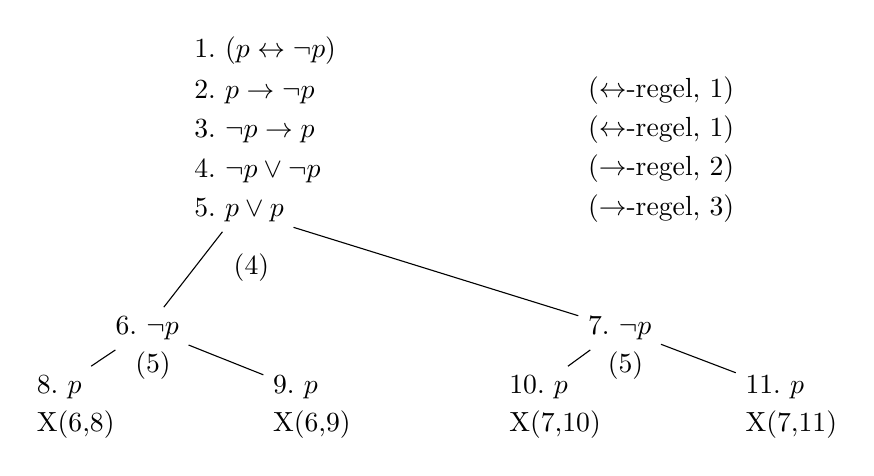
\begin{tikzpicture}[anchor=south west]
\node at (2,6) {$1.\ (p\leftrightarrow \neg p)$}; %\node at (7,6) {(formule)};
\node at (2,5.5) {$2.\ p\rightarrow \neg p$}; \node at (7,5.5) {($\leftrightarrow$-regel, 1)};
\node at (2,5) {$3.\ \neg p\rightarrow p$}; \node at (7,5) {($\leftrightarrow$-regel, 1)};
\node at (2,4.5) {$4.\ \neg p \lor  \neg p$}; \node at (7,4.5) {($\rightarrow$-regel, 2)};
\node at (2,4) (p1) {$5.\ p\lor p$}; \node at (7,4) {($\rightarrow$-regel, 3)};
\node at (1,2.5) (p2) {$6.\  \neg p$}; \node at (7,2.5) (p3) {$7.\ \neg p$};
\draw (p2) -- (p1) -- (p3);
\node at (2.5, 3.25) {$(4)$};
\node at (0, 1.75) (p4) {$8.\ p$}; \node at (3, 1.75) (p5) {$9.\ p$}; \node at (6,1.75) (p6) {$10.\ p$}; \node at (9,1.75) (p7) {$11.\ p$};
\draw (p4) -- (p2) -- (p5); \draw (p6) -- (p3) -- (p7);
\node at (1.25, 2) {$(5)$}; \node at (7.25, 2) {$(5)$};
\node at (0,1.25) {X(6,8)}; \node at (3, 1.25) {X(6,9)}; \node at (6,1.25) {X(7,10)}; \node at (9, 1.25) {X(7,11)};

\end{tikzpicture}
\end{center}
Alle takken van de boom sluiten, dus $p\leftrightarrow\neg p$ is onvervulbaar, dat wil zeggen $p\leftrightarrow\neg p$ is een contradictie.
\end{enumerate}
\end{answer}

\begin{answer} % 3.3
Bewijs met de boommethode dat:
\begin{enumerate}[label=\textit{\alph*.}]
%a
\item $p, (p\land\neg q)\rightarrow r, \neg (p\land r)\vdash q$. \\
antwoord:
Om de geldigheid te testen kunnen we kijken of de negatie van de conclusie vervulbaar is of niet.
\begin{center}
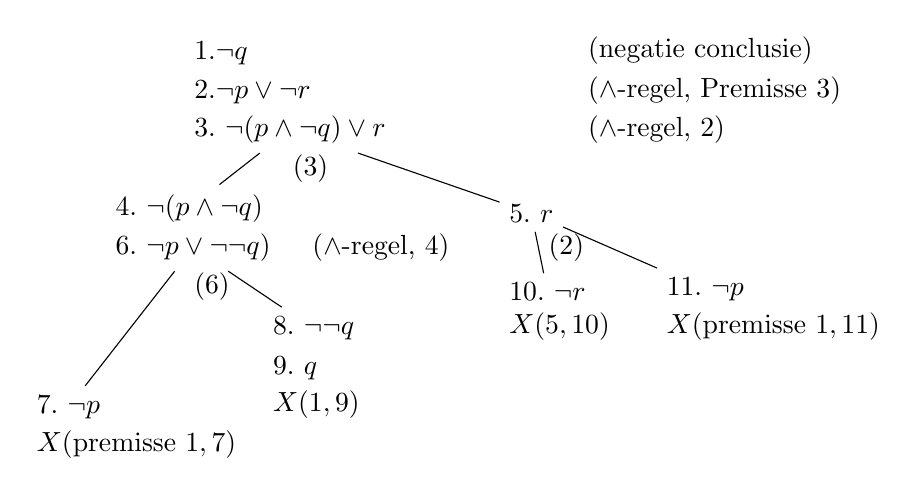
\begin{tikzpicture}[anchor=south west]
\node at (2,5.5) {$1. \neg q $}; \node at (7,5.5) {(negatie conclusie)};
\node at (2,5) {$2. \neg p \lor \neg r$}; \node at (7,5) {($\land$-regel, Premisse 3)};
\node at (2,4.5) (p1) {$3.\ \neg (p\land \neg q)\lor r$}; \node at (7,4.5) {($\land$-regel, 2)};
%branching
\node at (1, 3.5) (p2) {$4.\ \neg (p\land \neg q)$}; 
\node at (6, 3.5) (p3) {$5.\ r$};
\draw (p2) -- (p1) -- (p3);
\node at (3.25, 4) {$(3)$};
%branch 1:
\node at (1, 3)(p4) {$6.\ \neg p\lor\neg\neg q)$}; \node at (3.5, 3) {($\land$-regel, 4)};
%branching:
\node at (0, 1) (p5) {$7.\ \neg p$}; 
\node at (3, 2) (p6) {$8.\ \neg\neg q$};
\draw (p5) -- (p4) -- (p6);
\node at (2, 2.5) {$(6)$};
%branch 3:
\node at (0, 0.5) {$X($premisse 1$, 7)$};
%branch 4:
\node at (3, 1.5) {$9.\ q$};
\node at (3, 1) {$X(1,9)$};
 
%branch 2:
%branching
\node at (6, 2.5) (p7) {$10.\ \neg r$}; 
\node at (8, 2.5) (p8) {$11.\ \neg p$};
\draw (p7) -- (p3) -- (p8);
\node at (6.5, 3) {$(2)$};

\node at (6, 2)  {$X(5,10)$}; 

\node at (8, 2) {$X($premisse 1$,11)$}; 


\end{tikzpicture}
\end{center}
De verzameling met de negatie van de conclusie en de premissen is onvervulbaar. Dit betekent dat er geen enkele invulling is, gegeven de premissen, waarbij $\neg q$ waar is. Er is dus geen tegenvoorbeeld. Hiermee is bewezen dat de redenering logisch geldig is.
% b:
\item $\neg p\leftrightarrow(q\lor r), p\land r\vdash\neg q$.\\
antwoord:
\begin{center}
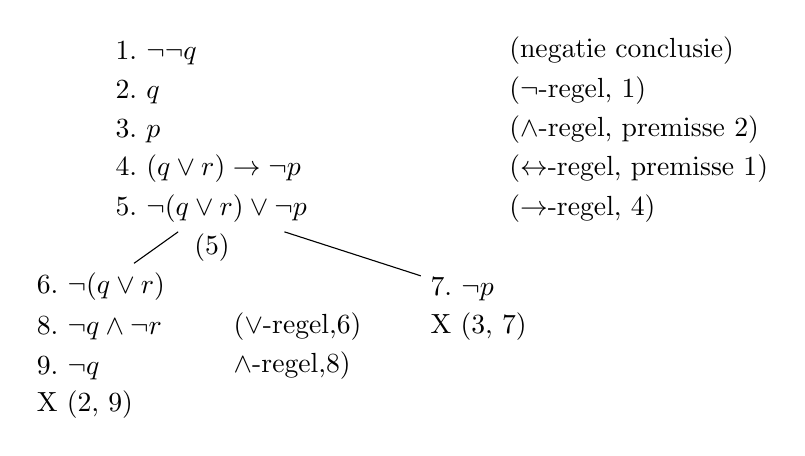
\begin{tikzpicture}[anchor=south west]
\node at (2,5.5) {$1.\ \neg \neg q$}; \node at (7,5.5) {(negatie conclusie)};
\node at (2, 5) {$2.\ q$}; \node at (7,5) {($\neg$-regel, 1)};
\node at (2, 4.5) {$3.\ p$}; \node at (7,4.5) {($\wedge$-regel, premisse 2)};
\node at (2, 4) {$4.\ (q\vee r)\rightarrow\neg p$}; \node at (7,4) {($\leftrightarrow$-regel, premisse 1)};
\node at (2, 3.5) (p1) {$5.\ \neg(q\vee r)\vee\neg p$}; \node at (7,3.5) {($\rightarrow$-regel, 4)};
\node at (1, 2.5) (p2) {$6.\ \neg(q\vee r)$}; \node at (6, 2.5) (p3) {$7.\ \neg p$};
\draw (p2) -- (p1) -- (p3);
\node at (3, 3) {$(5)$};
 %% branch 1
\node at (1,2) {$8.\ \neg q\wedge\neg r$}; \node at (3.5, 2) {($\vee$-regel,6)};
\node at (1, 1.5) {$9.\ \neg q$}; \node at (3.5, 1.5) {$\wedge$-regel,8)};
\node at (1, 1) {X (2, 9)};
 %% branch 2
 \node at (6, 2) {X (3, 7)};
\end{tikzpicture}
\end{center}
Alle takken sluiten, dus $\neg q$ volgt logisch uit $\neg p\leftrightarrow (q\vee r), p\wedge r$.
% c:
\item $p\leftrightarrow(\neg q\lor\neg r), \neg(\neg p\rightarrow r)\vdash \neg q$.\\
antwoord:
We gaan kijken of we een tegenvoorbeeld kunnen construeren door de vervulbaarheid van de negatie van de conclusie te testen.
\begin{center}
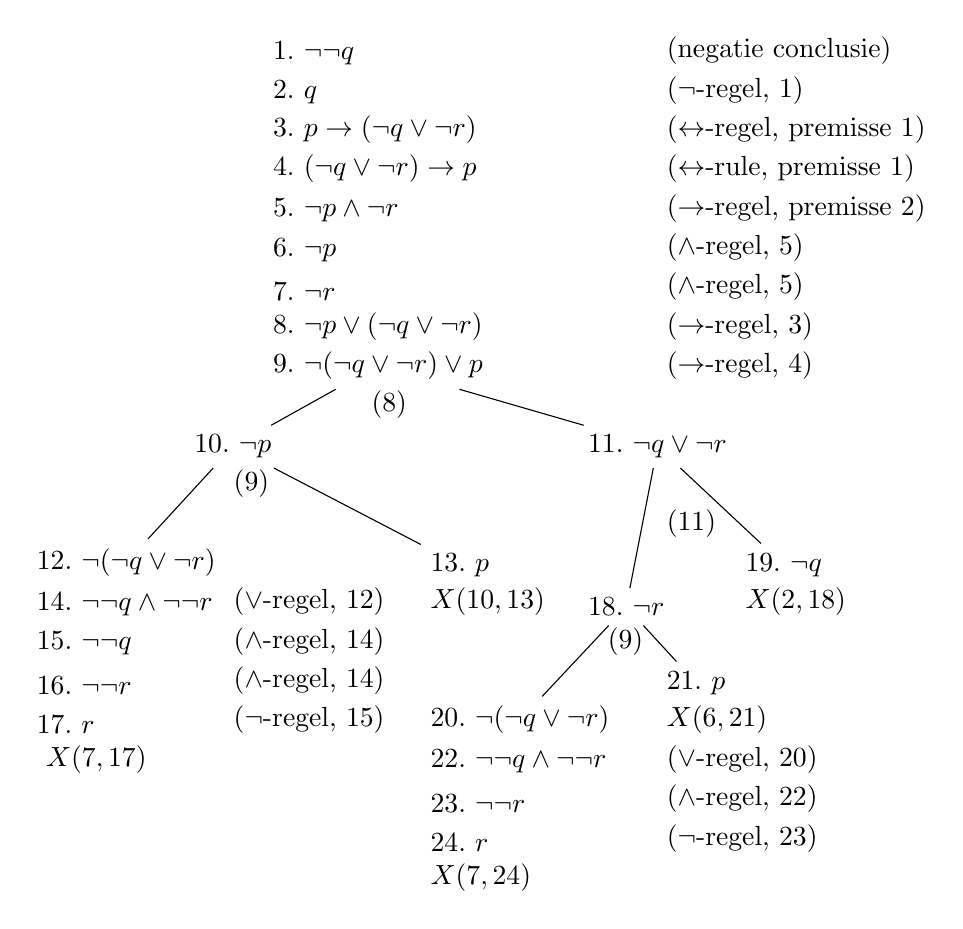
\begin{tikzpicture}[anchor=south west]
\node at (2,5.5) {$1.\ \neg \neg q$}; \node at (7,5.5) {(negatie conclusie)};
\node at (2, 5) {$2.\ q$}; \node at (7,5) {($\neg$-regel, 1)};
\node at (2, 4.5) {$3.\ p \rightarrow (\neg q \lor \neg r)$}; \node at (7,4.5) {($\leftrightarrow$-regel, premisse 1)};
\node at (2, 4) {$4.\ (\neg q\lor\neg r) \rightarrow p$}; \node at (7,4) {($\leftrightarrow$-rule, premisse 1)};
\node at (2,3.5) {$5.\ \neg p \land\neg r$}; \node at (7,3.5) {($\rightarrow$-regel, premisse 2)};
\node at (2, 3) {$6.\ \neg p$}; \node at (7,3) {($\land$-regel, 5)};
\node at (2, 2.5) {$7.\ \neg r$}; \node at (7,2.5) {($\land$-regel, 5)};
\node at (2, 2) (p1) {$8.\ \neg p \lor(\neg q\lor\neg r)$}; \node at (7,2) {($\rightarrow$-regel, 3)};
\node at (2, 1.5) (p1) {$9.\ \neg (\neg q\lor\neg r) \lor p$}; \node at (7,1.5) {($\rightarrow$-regel, 4)};
\node at (1, 0.5) (p2) {$10.\ \neg p$}; \node at (6, 0.5) (p3) {$11.\ \neg q\vee \neg r$};
\draw (p2) -- (p1) -- (p3);
\node at (3.25, 1) {$(8)$};
\node at (-1,-1) (p4) {$12.\ \neg (\neg q \lor \neg r)$};
\node at (4,-1) (p5) {$13.\ p$};
\draw (p4) -- (p2) -- (p5);
\node at (4,-1.5) (p5) {$X(10,13)$};
\node at (-1,-1.5) (p4) {$14.\ \neg\neg q\land \neg\neg r$}; \node at (1.5,-1.5) {($\lor$-regel, 12)};
\node at (1.5, 0) {$(9)$};

\node at (-1,-2) (p4) {$15.\ \neg\neg q$}; \node at (1.5,-2) {($\land$-regel, 14)};
\node at (-1,-2.5) (p4) {$16.\ \neg\neg r$}; \node at (1.5,-2.5) {($\land$-regel, 14)};
\node at (-1,-3) (p4) {$17.\ r$}; \node at (1.5,-3) {($\neg$-regel, 15)};
\node at (-1,-3.5) (p4) {$\ X(7,17)$}; 

\node at (6, -1.5) (p6) {$18.\ \neg r$};
\node at (8, -1) (p7) {$19.\ \neg q$};
\node at (8, -1.5) {$X(2,18)$};
\draw (p6) -- (p3) -- (p7);
\node at (7, -0.5) {$(11)$};

\node at (4, -3) (p8) {$20.\ \neg (\neg q \lor \neg r)$};
\node at (7, -2.5) (p9) {$21.\ p$};
\node at (7, -3) {$X(6,21)$};
\draw (p8) -- (p6) -- (p9);
\node at (6.25, -2) {$(9)$};
\node at (4, -3.5) {$22.\ \neg\neg q \land \neg\neg r$}; \node at (7, -3.5) {($\lor$-regel, 20)};
\node at (4, -4) {$23.\ \neg\neg r$}; \node at (7, -4) {($\land$-regel, 22)};
\node at (4, -4.5) {$24.\ r$}; \node at (7, -4.5) {($\neg$-regel, 23)};
\node at (4, -5) {$X(7,24)$};
\end{tikzpicture}
\end{center}
Alle takken van de boom sluiten. Dit betekent dat de negatie van de conclusie onvervulbaar is en we geen tegenvoorbeeld kunnen construeren. De redenering is dus logisch geldig.
% d:
\item $p\rightarrow((q\rightarrow r)\rightarrow s), \neg(p\rightarrow s)\vdash\neg(q\rightarrow r)$. \\
antwoord: \\
We gaan kijken of we een tegenvoorbeeld kunnen construeren door de vervulbaarheid de verzameling van de negatie van de conclusie en de premissen te testen.

\begin{center}
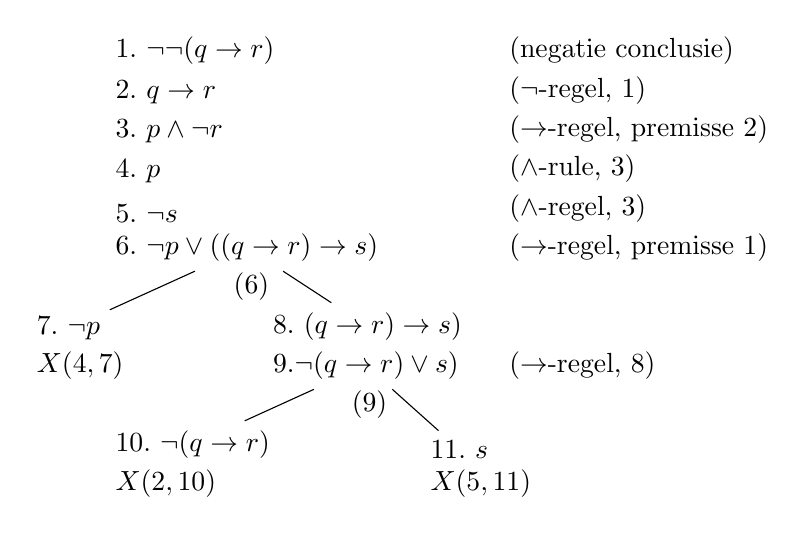
\begin{tikzpicture}[anchor=south west]
\node at (2,5.5) {$1.\ \neg \neg (q\rightarrow r)$}; \node at (7,5.5) {(negatie conclusie)};
\node at (2, 5) {$2.\ q \rightarrow r$}; \node at (7,5) {($\neg$-regel, 1)};
\node at (2, 4.5) {$3.\ p\land\neg r$}; \node at (7,4.5) {($\rightarrow$-regel, premisse 2)};
\node at (2, 4) {$4.\ p$}; \node at (7,4) {($\land$-rule, 3)};
\node at (2,3.5) {$5.\ \neg s$}; \node at (7,3.5) {($\land$-regel, 3)};
\node at (2, 3) (p1) {$6.\ \neg p\lor((q\rightarrow r)\rightarrow s)$}; \node at (7,3) {($\rightarrow$-regel, premisse 1)};
\node at (1, 2) (p2) {$7.\ \neg p$}; 
\node at (4, 2) (p3) {$8.\ (q\rightarrow r)\rightarrow s)$};
\draw (p2) -- (p1) -- (p3);
\node at (3.5, 2.5) {$(6)$};
\node at (1, 1.5){$X(4,7)$};

\node at (4, 1.5)(p4) {$9.\neg (q\rightarrow r)\lor s)$}; \node at (7, 1.5) {($\rightarrow$-regel, 8)};
\node at (2, 0.5)(p5) {$10.\ \neg(q\rightarrow r)$};
\node at (6, 0.5)(p6) {$11.\  s$};
\draw (p5) -- (p4) -- (p6);
\node at (5, 1) {$(9)$};

\node at (6, 0.0) {$X(5,11)$};

\node at (2, 0.0) {$X(2,10)$};
\end{tikzpicture}
\end{center}
Alle takken van de boom sluiten. Dit betekent dat de negatie van de conclusie, in combinatie met de premissen, onvervulbaar is en we geen tegenvoorbeeld kunnen construeren. De redenering is dus logisch geldig.

%e:
\item $(p\land q)\rightarrow r,\neg p\lor(p\rightarrow q)\vdash p\rightarrow r$.\\
antwoord: om te bewijzen dat de redenering logisch geldig is, gaan we kijken of we een tegenvoorbeeld kunnen construeren. Dit doen we door te kijken of de negatie van de conclusie vervulbaar is.
\begin{center}
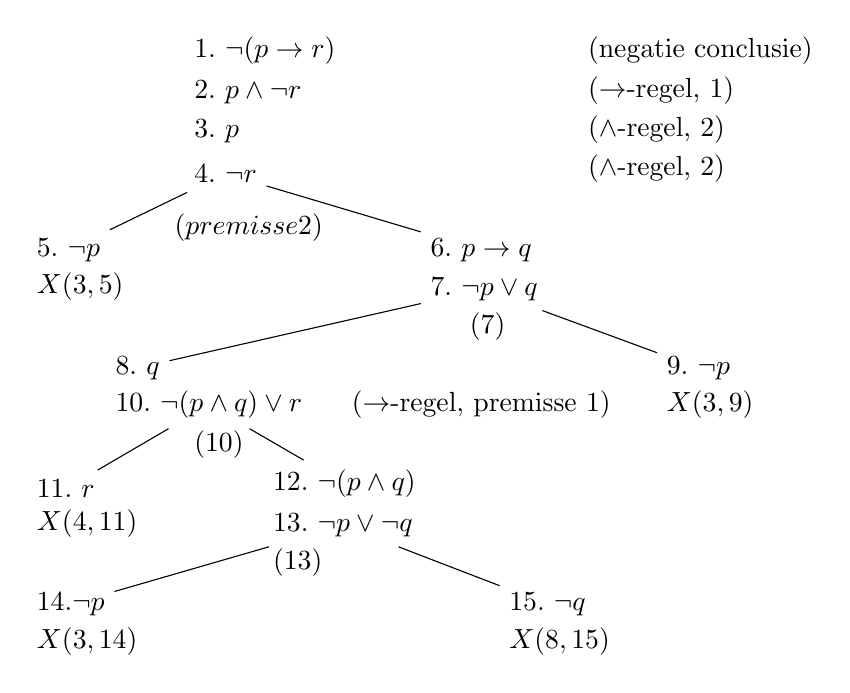
\begin{tikzpicture}[anchor=south west]
\node at (2,7) {$1.\ \neg (p\rightarrow r)$}; \node at (7,7) {(negatie conclusie)};
\node at (2,6.5) {$2.\ p\land\neg r$}; \node at (7,6.5) {($\rightarrow$-regel, 1)};
\node at (2,6) {$3.\ p$}; \node at (7,6) {($\land$-regel, 2)};

\node at (2,5.5)(p1) {$4.\ \neg r$}; \node at (7,5.5) {($\land$-regel, 2)};
%branching
\node at (0, 4.5) (p2) {$5.\ \neg p$}; 
\node at (5, 4.5) (p3) {$6.\ p\rightarrow q$};
\draw (p2) -- (p1) -- (p3);
\node at (1.75, 4.75) {$(premisse 2)$};
%branch 1
\node at (0, 4) {$X(3,5)$};
%branch 2:
\node at (5, 4) (p4) {$7.\ \neg p\lor q$};
%branching
\node at (1, 3) (p5) {$8.\ q$};
\node at (8, 3) (p6) {$9.\ \neg p$}; 
\draw (p5) -- (p4) -- (p6);
\node at (5.5, 3.5) {$(7)$};
%branch 3:
\node at (8, 2.5) {$X(3,9)$};
%branch 4:
\node at (1, 2.5) (p7) {$10.\ \neg(p \land q) \lor r$}; \node at (4, 2.5) {($\rightarrow$-regel, premisse 1)};
%branching
\node at (0, 1.5) (p8) {$11.\ r$};
\node at (3, 1.5) (p9) {$12.\ \neg(p \land q)$}; 
\draw (p8) -- (p7) -- (p9);
\node at (2, 2) {$(10)$};
%branch 5:
\node at (0, 1) {$X(4,11)$};
%branch 6:
\node at (3, 1)(p10) {$13.\ \neg p \lor\neg q$};

%branching:
\node at (0, 0) (p11) {$14.\neg p$};
\node at (6, 0) (p12) {$15.\ \neg q$}; 
\draw (p11) -- (p10) -- (p12);
\node at (3, 0.5) {$(13)$};
%branch 7:
\node at (0, -0.5) {$X(3,14)$};
%branch 8:
\node at (6, -0.5) {$X(8,15)$};

\end{tikzpicture}
\end{center}

%f:
\item $(p\rightarrow\neg r)\lor(p\rightarrow q), r\rightarrow p\vdash r\rightarrow q$.\\
antwoord: We gaan kijken of we een bewijs kunnen vinden door de onvervulbaarheid van de negatie van de conclusie af te leiden:
\begin{adjustwidth}{-2em}{}
\begin{center}
    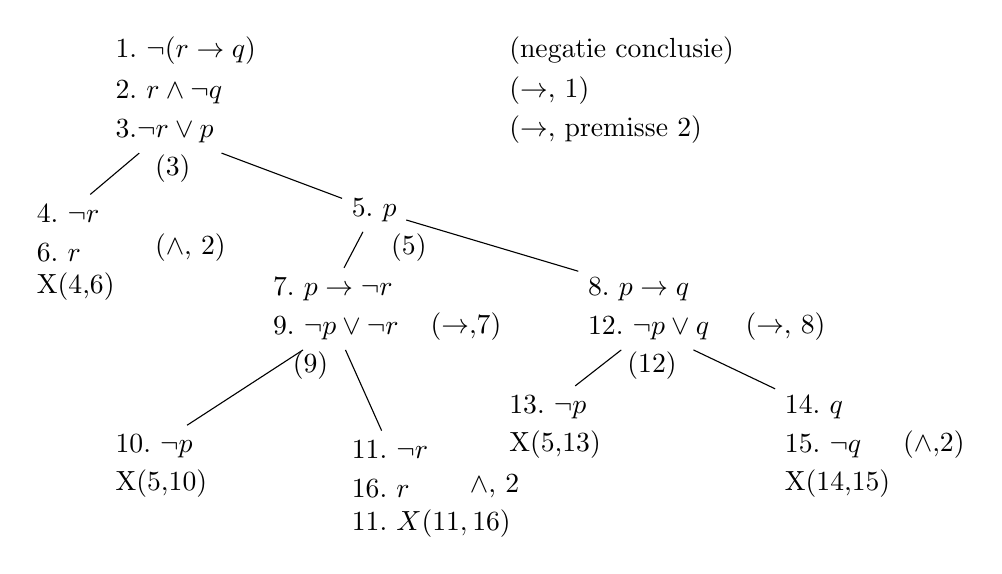
\begin{tikzpicture}[anchor=south west]
    \node at (2,7) {$1.\ \neg(r\rightarrow q)$}; \node at (7,7) {(negatie conclusie)};
    \node at (2, 6.5) {$2.\ r\wedge\neg q$}; \node at (7, 6.5) {($\rightarrow$, 1)};
    \node at (2, 6) (p1) {$3. \neg r\vee p$}; \node at (7, 6) {($\rightarrow$, premisse 2)};
    \node at (1,5) (p2) {$4.\ \neg r$}; \node at (5,5) (p3) {$5.\ p$};
    \draw (p2) -- (p1) -- (p3);
    \node at (2.5, 5.5) {$(3)$};
    %% left branch
    \node at (1,4.5) {$6.\ r$}; \node at (2.5,4.5) {($\wedge$, 2)};
    \node at (1, 4) {X(4,6)};
    % right branch
    \node at (4,4) (p4) {$7.\ p\rightarrow \neg r$}; \node at (8, 4) (p5) {$8.\ p\rightarrow q$};
    \draw (p4) -- (p3) -- (p5);
    \node at (5.5, 4.5) {$(5)$};
    %right, left branch
    \node at (4, 3.5) (p6) {$9.\ \neg p\vee \neg r$}; \node at (6, 3.5) {($\rightarrow$,7)};
    \node at (2, 2) (p7) {$10.\ \neg p$}; \node at (5,2) (p8) {$11.\ \neg r$};
    \draw (p7) -- (p6) -- (p8);
    \node at (4.25, 3) {$(9)$};
    \node at (2, 1.5) {X(5,10)};
    \node at (5,1.5) {$16.\ r$};\node at (6.5,1.5) {$\land$, 2};
    \node at (5,1) {$11.\ X(11,16)$};
    %right, right branch
    \node at (8, 3.5) (p9) {$12.\ \neg p\vee q$};\node at (10, 3.5) {($\rightarrow$, 8)};
    \node at (7, 2.5) (p10) {$13.\ \neg p$}; \node at (10.5, 2.5) (p11) {$14.\ q$};
    \draw (p10) -- (p9) -- (p11);
    \node at (8.5, 3) {$(12)$};
    \node at (7, 2) {X(5,13)};
    \node at (10.5, 2) {$15.\ \neg q$};\node at (12,2) {($\wedge$,2)};
    \node at (10.5,1.5) {X(14,15)};
    \end{tikzpicture}
\end{center}
\end{adjustwidth}
Allen takken sluiten, dus het logisch gevolg is geldig. 
\end{enumerate}
\end{answer}


\begin{answer} % 3.4
Ga voor elk van de onderstaande beweringen na of deze juist dan wel onjuist is. Geef in het eerste geval een bewijs met behulp van de boommethode. Construeer in het tweede geval een \textit{tegenvoorbeeld}.
\begin{enumerate}[label=\textit{\alph*.}]
\item $p\rightarrow q,\neg r\rightarrow q\vdash p\rightarrow r$.\\
Antwoord: we bekijken of het logisch gevolg geldt door de vervulbaarheid te inspecteren van de premissen en de negatie van de conclusie:
\begin{center}
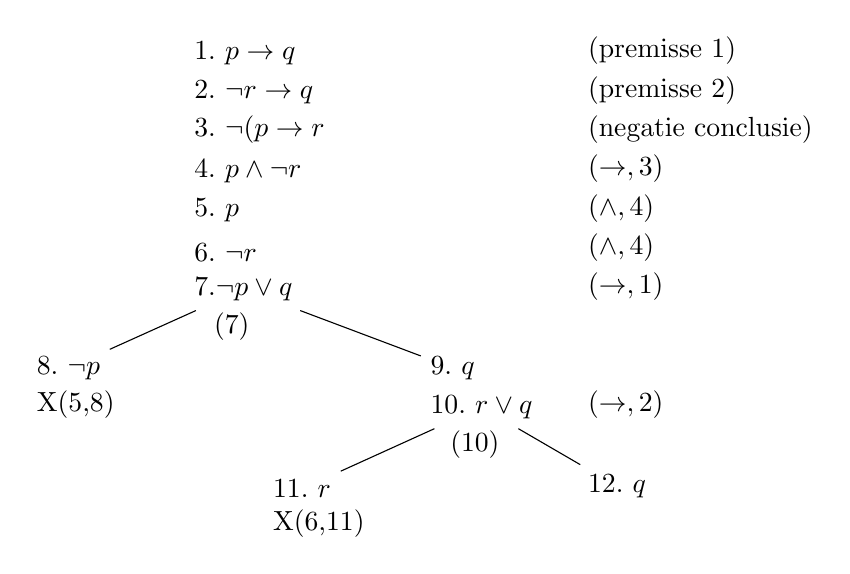
\begin{tikzpicture}[anchor=south west]
\node at (2,8) {$1.\ p\rightarrow q$};\node at (7,8) {(premisse 1)};
\node at (2,7.5) {$2.\ \neg r\rightarrow q$};\node at (7,7.5) {(premisse 2)};
\node at (2,7) {$3.\ \neg(p\rightarrow r$};\node at (7,7) {(negatie conclusie)};
\node at (2,6.5) {$4.\ p\wedge\neg r$};\node at (7,6.5) {$(\rightarrow, 3)$};
\node at (2, 6) {$5.\ p$};\node at (7,6) {$(\wedge, 4)$};
\node at (2, 5.5) {$6.\ \neg r$};\node at (7,5.5) {$(\wedge, 4)$};
\node at (2,5) (p1) {$7.\neg p\vee q$};\node at (7,5) {$(\rightarrow, 1)$};
\node at (0, 4) (p2) {$8.\ \neg p$}; \node at (5, 4) (p3) {$9.\ q$};
\draw (p2) -- (p1) -- (p3);
\node at (2.25,4.5) {$(7)$};
\node at (0, 3.5) {X(5,8)};
\node at (5,3.5) (p4) {$10.\ r\vee q$};\node at (7,3.5) {$(\rightarrow, 2)$};
\node at (3, 2.5) (p5) {$11.\ r$}; \node at (7, 2.5) (p6) {$12.\ q$}; 
\draw (p5) -- (p4) -- (p6);
\node at (5.25, 3) {$(10)$};
\node at (3, 2) {X(6,11)};
\end{tikzpicture}
\end{center}
Er is een tak die niet sluit, dus de premissen zijn vervulbaar in combinatie met de negatie van de conclusie. Het logisch gevolg is derhalve niet geldig. Een tegenvoorbeeld is wanneer $p=1$, $q=1$ en $r=0$.
\item $\vdash ((p\lor(p\rightarrow q))\rightarrow q)\rightarrow q$.\\
Antwoord: Wederom verifi\"eren we de vervulbaarheid van de premissen en de negatie van de conclusie:
\begin{center}
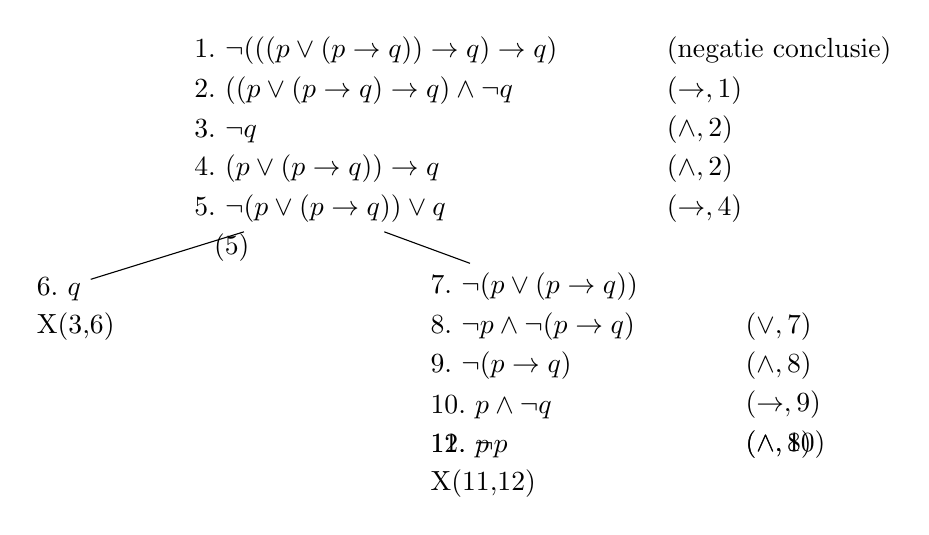
\begin{tikzpicture}[anchor=south west]
\node at (2,8) {$1.\ \neg (((p\vee (p\rightarrow q))\rightarrow q)\rightarrow q)$};\node at (8,8) {(negatie conclusie)};
\node at (2,7.5) {$2.\ ((p\vee(p\rightarrow q)\rightarrow q)\wedge\neg q$};\node at (8,7.5) {$(\rightarrow, 1)$};
\node at (2,7) {$3.\ \neg q$};\node at (8,7) {$(\wedge,2)$};
\node at (2,6.5) {$4.\ (p\vee(p\rightarrow q))\rightarrow q$};\node at (8,6.5) {$(\wedge,2)$};
\node at (2,6) (p1) {$5.\ \neg(p\vee(p\rightarrow q))\vee q$};\node at (8,6) {$(\rightarrow, 4)$};
\node at (0,5) (p2) {$6.\ q$}; \node at (5,5) (p3) {$7.\ \neg(p\vee(p\rightarrow q))$};
\draw (p2) -- (p1) -- (p3);
\node at (2.25, 5.5) {$(5)$};
\node at (0,4.5) {X(3,6)};
\node at (5,4.5) {$8.\ \neg p\wedge\neg (p\rightarrow q)$};\node at (9,4.5) {$(\vee,7)$};
\node at (5, 4) {$9.\ \neg(p\rightarrow q)$};\node at (9,4) {$(\wedge,8)$};
\node at (5,3.5) {$10.\ p\wedge\neg q$};\node at (9,3.5) {$(\rightarrow, 9)$};
\node at(5,3) {$11.\ p$};\node at (9,3) {$(\wedge,10)$};
\node at(5,3) {$12.\ \neg p$};\node at (9,3) {$(\wedge,8)$};
\node at (5,2.5) {X(11,12)};
\end{tikzpicture}
\end{center}
Alle takken sluiten, dus het logisch gevolg is geldig.
\item $(p\land q)\rightarrow s, \neg(s\rightarrow t), q\lor t\vdash \neg p$.\\
Antwoord: Wederom verifi\"eren we de vervulbaarheid van de premissen en de negatie van de conclusie:
\begin{center}
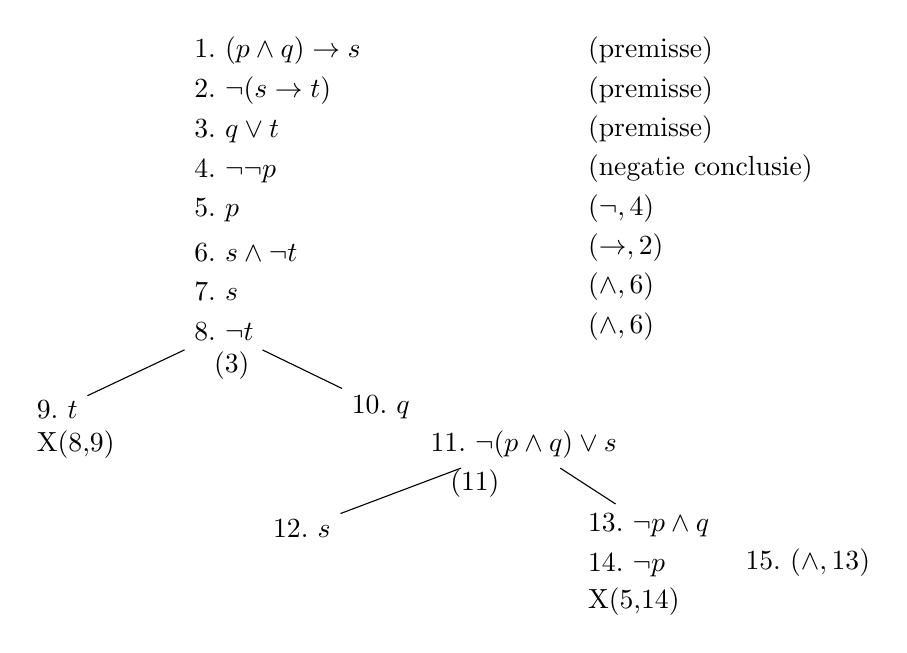
\begin{tikzpicture}[anchor=south west]
\node at (2,8) {$1.\ (p\wedge q)\rightarrow s$};\node at (7,8) {(premisse)};
\node at (2,7.5) {$2.\ \neg (s\rightarrow t)$};\node at (7,7.5) {(premisse)};
\node at (2,7) {$3.\ q\vee t$};\node at (7,7) {(premisse)};
\node at (2,6.5) {$4.\ \neg\neg p$};\node at (7,6.5) {(negatie conclusie)};
\node at (2,6) {$5.\ p$};\node at (7,6) {$(\neg, 4)$};
\node at (2,5.5) {$6.\ s\wedge\neg t$};\node at (7,5.5) {$(\rightarrow,2)$};
\node at (2,5) {$7.\ s$};\node at (7,5) {$(\wedge,6)$};
\node at (2,4.5) (p) {$8.\ \neg t$};\node at (7,4.5) {$(\wedge, 6)$};
\node at (0, 3.5) (q) {$9.\ t$}; \node at (4,3.5) (r) {$10.\ q$};
\draw (q) -- (p) -- (r);
\node at (2.25,4) {$(3)$};
\node at (0, 3) {X(8,9)};
\node at (5,3) (u) {$11.\ \neg(p\wedge q)\vee s$};
\node at (3, 2) (v) {$12.\ s$}; \node at (7,2) (w) {$13.\ \neg p\wedge q$};
\draw (v) -- (u) -- (w);
\node at (5.25,2.5) {$(11)$};
\node at (7,1.5) {$14.\ \neg p$}; \node at (9, 1.5) {$15.\ (\wedge, 13)$};
\node at (7,1) {X(5,14)};
\end{tikzpicture}
\end{center}
E\'en tak (bij regel 12) sluit niet, dus de premissen zijn vervulbaar samen met de negatie van de conclusie. Daarom is het logisch gevolg niet geldig.
\item $\neg p\rightarrow p\vdash p$.\\
Antwoord: Wederom verifi\"eren we de vervulbaarheid van de premissen en de negatie van de conclusie:
\begin{center}
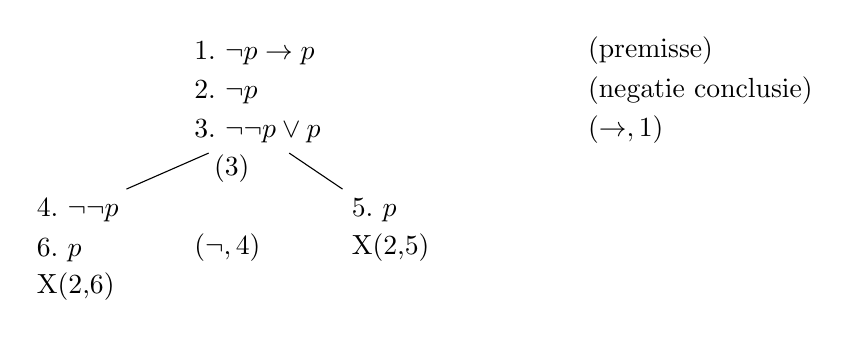
\begin{tikzpicture}[anchor=south west]
\node at (2,5) {$1.\ \neg p\rightarrow p$};\node at (7,5) {(premisse)};
\node at (2,4.5) {$2.\ \neg p$};\node at (7,4.5) {(negatie conclusie)};
\node at (2,4) (p) {$3.\ \neg\neg p\vee p$};\node at (7,4) {$(\rightarrow, 1)$};
\node at (0,3) (q) {$4.\ \neg\neg p$};\node at (4,3) (r) {$5.\ p$};
\draw (q) -- (p) -- (r);
\node at (2.25,3.5) {$(3)$};
\node at (0,2.5) {$6.\ p$};\node at (2,2.5) {$(\neg, 4)$};\node at (4,2.5) {X(2,5)};
\node at (0,2) {X(2,6)};
\end{tikzpicture}
\end{center}
Alle takken van de boom sluiten, dus het gegeven logische gevolg is geldig.
\item $\vdash (p\lor q)\rightarrow (p\land q)$.\\
Antwoord: Wederom verifi\"eren we de vervulbaarheid van de premissen en de negatie van de conclusie:
\begin{center}
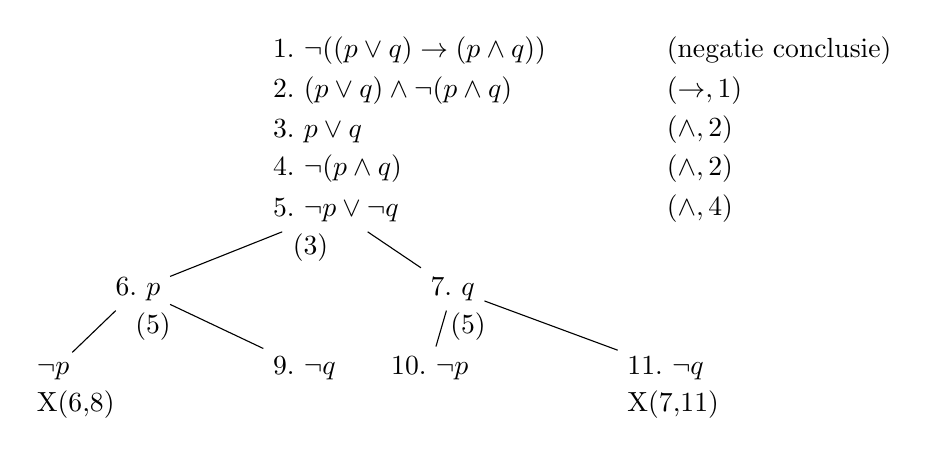
\begin{tikzpicture}[anchor=south west]
\node at (2,7) {$1.\ \neg((p\vee q)\rightarrow (p\wedge q))$};\node at (7,7) {(negatie conclusie)};
\node at (2,6.5) {$2.\ (p\vee q)\wedge\neg(p\wedge q)$};\node at (7,6.5) {$(\rightarrow, 1)$};
\node at (2,6) {$3.\ p\vee q$};\node at (7,6) {$(\wedge,2)$};
\node at (2,5.5) {$4.\ \neg (p\wedge q)$};\node at (7,5.5) {$(\wedge, 2)$};
\node at (2,5) (p) {$5.\ \neg p\vee\neg q$};\node at (7,5) {$(\wedge, 4)$};
\node at (0,4) (q) {$6.\ p$};\node at (4,4) (r) {$7.\ q$};
\draw (q) -- (p) -- (r);
\node at (2.25,4.5) {$(3)$};
\node at (-1, 3) (u) {$\neg p$};\node at (2,3) (v) {$9.\ \neg q$};\node at (3.5, 3) (w) {$10.\ \neg p$};\node at (6.5,3) (x) {$11.\ \neg q$};
\draw (u) -- (q) -- (v);
\node at (0.25,3.5) {$(5)$};\node at (4.25,3.5) {$(5)$};
\draw (w) -- (r) -- (x);
\node at (-1, 2.5) {X(6,8)}; \node at (6.5,2.5) {X(7,11)};
\end{tikzpicture}
\end{center}
Niet alle takken de boom sluiten, dus het logisch gevolg is niet geldig.
\item $\neg p,p\vdash q$.\\
Antwoord: Wederom verifi\"eren we de vervulbaarheid van de premissen en de negatie van de conclusie:
\begin{center}
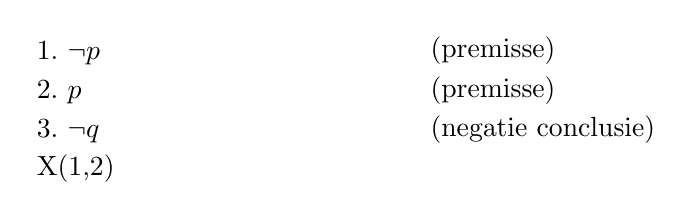
\begin{tikzpicture}[anchor=south west]
\node at (2,3) {$1.\ \neg p$};\node at (7,3) {(premisse)};
\node at (2,2.5) {$2.\ p$};\node at (7,2.5) {(premisse)};
\node at (2,2) {$3.\ \neg q$};\node at (7,2) {(negatie conclusie)};
\node at (2,1.5) {X(1,2)};
\end{tikzpicture}
\end{center}
Alle takken van de boom sluiten, dus het logisch gevolg is geldig.
\end{enumerate}
\end{answer}

\newpage
\begin{answer} % 3.5
Vertaal de volgende redeneringen naar \textit{propositielogica} en ga met behulp van de boommethode na of deze logisch geldig zijn of niet. Produceer in het laatste geval ook een tegenvoorbeeld.
\begin{enumerate}[label=\textit{\alph*.}]
\item \textit{Als Tom nuchter is, dan handelt hij rationeel maar hij is dan wel oninteressant.}\\
\textit{Als hij beleefd en oninteressant is, dan vindt Sylvia hem niet aardig.}\\
\textit{Dus, als Tom nuchter en beleefd is, dan vindt Sylvia hem niet aardig.}\\
Antwoord: Wederom verifi\"eren we de vervulbaarheid van de premissen en de negatie van de conclusie:\\
    $n$: Tom is nuchter, $r$: Tom is rationeel, $i$: Tom is interessant, $b$: Tom is beleefd, $s$: Sylvia vindt Tom aardig.
\begin{center}
\begin{tableau}{line no sep= 5mm,for tree={s sep'=5mm}}
[ n \to (r \land \neg i),                 just={Premisse 1}
[ (b \land \neg i) \to \neg s,            just={Premisse 2}
[ \neg ((n \land b) \to \neg s),          just={Negatie conclusie}
[ \neg n \lor (r \land \neg i),           just={$\to$-regel, 1}
[ \neg(b \land \neg i) \lor \neg s,       just={$\to$-regel, 2}
[ (n \land b) \land \neg (\neg s),        just={$\to$-regel, 3}
[ n \land b,                              just={$\land$-regel, 6}
[ \neg (\neg s),                          just={$\land$-regel, 6}
[ n,                                      just={$\land$-regel, 7}
[ b,                                      just={$\land$-regel, 7}
[ s,                                      just={$\neg$-regel, 8}
  [ \neg (b \land \neg i),                just={$\lor$-regel, 5}
  [ \neg b \lor \neg (\neg i),            just={$\land$-regel, 12}
    [ \neg b,                             just={$\lor$-regel, 13}
      [ \bot (10;14) ]
    ]
    [ \neg (\neg i)
    [ i,                                  just={$\neg$-regel, 14}
      [ \neg n,                           just={$\lor$-regel, 4}
        [ \bot(9; 16) ]
      ]
      [ r \land \neg i
      [ r,                                just={$\land$-regel, 16}
      [ \neg i,                           just={$\land$-regel, 16}
        [ \bot(15;18) ]
      ]]]
    ]]
  ]]
  [ \neg s [ \bot (11; 12)]
  ]
]]]]]]]]]]]
\end{tableau}\\[3mm]
Alle takken van de boom sluiten, dus het logisch gevolg is geldig.
\end{center}
\newpage
\item\textit{Als Anton lid wordt van de Nederlandse Vereniging van Terraszitters, dan worden Bob en Cees dat ook.}\\
\textit{Als Anton of Bob lid wordt, dan zal David zijn lidmaatschap opzeggen.}\\
\textit{Dus zal David zijn lidmaatschap opzeggen, ongeacht of Cees nou lid wordt of niet.}\\
Antwoord: Wederom verifi\"eren we de vervulbaarheid van de premissen en de negatie van de conclusie:\\
    $a$: Anton is (wordt of blijf) lid van de vereniging, $b$: Bert is lid van de vereniging, $c$: Cees is lid, $d$: David is lid.
\begin{center}
\begin{tableau}{line no sep= 5mm,for tree={s sep'=5mm}}
[ a \to (b \land c),               just={Premisse 1}
[ (a \lor b) \to \neg d,           just={Premisse 2}
[ \neg (\neg d),                   just={Negatie conclusie}
[ d,                               just={$\neg$-regel, 3}
[ \neg a \lor (b \land c),         just={$\to$-regel, 1}
[ \neg (a \lor b) \lor \neg d,     just={$\to$-regel, 2}
  [ \neg (a \lor b),               just={$\lor$-regel, 6}
  [ \neg a \land \neg b,           just={$\lor$-regel, 7}
  [ \neg a,                        just={$\land$-regel, 8}
  [ \neg b,                        just={$\land$-regel, 8}
    [ \neg a,                      just={$\lor$-regel, 5}
    ]
    [ b \land c
    [ b,                           just={$\land$-regel, 11}
    [ c,                           just={$\land$-regel, 11}
      [ \bot (10;12) ]]]]
  ]]]]
  [ \neg d
    [ \bot (4;7) ]
  ]]]]]]]
\end{tableau}\\[3mm]
Niet alle takken de boom sluiten, dus het logisch gevolg is niet geldig. Uit de boom valt een tegenvoorbeeld af te lezen, waarbij Anton en Bob geen lid worden en David lid blijft. Het maakt hierbij inderdaad niet uit wat Cees doet.
\end{center}

\newpage
\item\textit{Je kunt Hans geloven als je Bert kunt geloven, en omgekeerd.}\\
\textit{Als je noch Hans, noch Bert kunt geloven, dan kun je ook Greetje niet geloven.}\\
\textit{Je kunt Greetje geloven.}\\
\textit{Dus je kunt Bert geloven.}\\
Antwoord: Wederom verifi\"eren we de vervulbaarheid van de premissen en de negatie van de conclusie:\\
    $h$: Hans is geloofwaardig, $b$: Bert is geloofwaardig, $g$: Greetje is geloofwaardig.
\begin{center}
\begin{tableau}{line no sep= 5mm,for tree={s sep'=5mm}}
[ h \leftrightarrow b,                     just={Premisse 1}
[ (\neg h \land \neg b) \to \neg g,        just={Premisse 2}
[ g,                                       just={Premisse 3}
[ \neg b,                                  just={Negatie conclusie}
[ h \to b,                                 just={$\leftrightarrow$-regel, 1}
[ b \to h,                                 just={$\leftrightarrow$-regel, 1}
[ \neg h \lor b,                           just={$\to$-regel, 5}
[ \neg b \lor h,                           just={$\to$-regel, 5}
[ \neg (\neg h \land \neg b) \lor \neg g,  just={$\to$-regel, 2}
  [ \neg (\neg h \land \neg b),            just={$\lor$-regel, 9}
  [ \neg (\neg h) \lor \neg (\neg b),      just={$\land$-regel, 10}
    [ b,                                   just={$\lor$-regel, 7}
      [ \bot (4;12) ]
    ]
    [ \neg h
      [ \neg b,                            just={$\lor$-regel, 8}
        [ \neg (\neg h),                   just={$\lor$-regel, 11}
        [ h,                               just={$\neg$-regel, 16}
          [ \bot (12;17) ]
        ]]
        [ \neg (\neg b)
        [ b,                               just={$\neg$-regel, 16}
          [ \bot (4;17) ]
        ]]
      ]
      [ h
        [ \bot (12;14) ]
      ]
    ]
  ]]
  [ \neg g
    [ \bot (3;10) ]
  ]
]]]]]]]]]
\end{tableau}\\[3mm]
Alle takken van de boom sluiten, dus het logisch gevolg is geldig.
\end{center}
\end{enumerate}

\end{answer}
